% &LaTeX

\section{Feedback Filters}

By the end of this lab you should feel comfortable manipulating and
using feedback filters for simple algorithms. You should also be
comfortable with the concept of a filter with an Infinite Impulse
Response (IIR). All feedback filters have an infinite impulse response
and are also known as IIR filters. Feedback filters use the previous
outputs of the filter, feeding them back into the output of the
current sample. The ``fed back'' outputs are weighted by coefficients,
$a_\ell$.

\subsection{Lab Background}

Note that the J-DSP \block{Coeff.} block uses \emph{negative} values
for the $a_\ell$ (feedback) coefficients. In other words, in the text,
a second-order feedback filter's defining equation might be:
\begin{align}
  y[n] &= a_1 y[n-1] + a_2 y[n-2] + b_0 x[n] \label{eq:def} \\
  y[n] -a_1 y[n-1] - a_2 y[n-2]&=   b_0 x[n]
\end{align}
This yields the transfer function:
\begin{align}
  Y(z)(1 - a_1 z^{-1} - a_2 z^{-2}) &= b_0X(z) \\
  Y(z)/X(z) &= \frac{b_0}{1 - a_1 z^{-1} - a_2 z^{-2}} \\
  H(z) &= \frac{b_0}{1 - a_1 z^{-1} - a_2 z^{-2}} \label{eq:trans} 
\end{align}
However, in J-DSP, the coefficients used, rather than being the
$a_\ell$ from the defining equation~(\ref{eq:def}) are the
\emph{negative $a_\ell$} from the transfer
function~(\ref{eq:trans}). In other words, to properly define the above filter in J-DSP,
you will need to use the coefficients, $a[0]=1,a[1]=-a_1,a[2]=-a_2$, and $b[0]=b_0$. 
Note also that in this example the \block{Coeff.} block has
an $a[0]$ coefficient, which we will always leave as 1.0 (it's the
first ``1'' in the denominator of the transfer function).

\subsection{Feedback Filters as Recurrence Relations}

You may notice that the defining equation for a feedback filter is in
the form of a recurrence relation. In fact, we can use a feedback
filter to implement a recurrence relation if we set the input to be
an impulse, $x[n] = C \delta[n]$, with amplitude $C$ being the initial
value for the iteration. Let's start out with the Fibonacci sequence,
which you'll remember to be:
\begin{equation}
  F[n] = \left\{ \begin{array}{ll}
      1 & n < 2 \\
      F[n-1] + F[n-2] & n \geq 2
    \end{array} \right.
\end{equation}

We can rewrite this recurrence relation as:
\begin{equation}
  y[n] = y[n-1] + y[n-2] + x[n]
  \label{eq:fib}
\end{equation}
and we will get the Fibonacci sequence \emph{if} we input an impulse
(hence, the appearance of the $x[n]$ on the right hand side, which
serves only to initialize the filter). This is also a very good
demonstration of the first ``I'' in the acronym ``IIR'': the impulse
response of this filter has infinite duration.

\paragraph{Step 1.1} If we set $x[n]=\delta[n]$ in~(\ref{eq:fib}), we
should see that the impulse response of this filter is indeed the
Fibonacci sequence. Implement this filter in J-DSP and verify that its
impulse response is the Fibonacci sequence. What are the values of the
coefficients in the \block{Coeff.} block that you used?


\paragraph{Step 1.2} What is the value for $n=19$ given by the
\block{Plot} block?


\paragraph{Step 1.3} Is this filter stable?


\paragraph{Step 1.4} Let's do something similar with the recurrence
relation for computing the series $y[n] = 1/3^n$ in the text. Set the
coefficients for a feedback filter to implement equation~(5-42) in the
text, $y[n] = 1/3 y[n-1] + x[n]$. What are the J-DSP filter coefficients?


\paragraph{Step 1.5} What are the pole location(s) for this filter?


\paragraph{Step 1.6} Now use J-DSP to calculate the impulse repsonse.
Set the amplitude of the input impulse to be 0.99996. Is this filter stable? 
Is its impulse response consistent with the result of iterating equation~(5-42) in the notes?


\subsection{Telephone Touch Tone Dialing}
Telephone touch pads generate dual tone multi frequency (DTMF) signals
to dial a telephone. When any key is pressed, the tones of the
corresponding column and row in the table below are generated, hence
it is a ``dual tone'' code. As an example, pressing the 5 button
generates the tones 770Hz and 1336Hz summed together.

\begin{center}
  \begin{tabular}{l|ccc}
    & 1209Hz & 1336Hz & 1477Hz \\ \hline
    697Hz &   1    &   2    &   3    \\
    770Hz &   4    &   5    &   6    \\
    852Hz &   7    &   8    &   9    \\
    941Hz &   $\ast $    &   0    &   \#    
  \end{tabular}
\end{center}

The frequencies in the table above were chosen to avoid harmonics. No
frequency is a multiple of another, the difference between any two
frequencies does not equal any of the frequencies, and the sum of any
two frequencies does not equal any of the frequencies.\footnote{More
  information can be found at:
  \url{http://en.wikipedia.org/wiki/DTMF}} This makes it easier to
detect exactly which tones are present in the dial signal in the
presence of line distortions.

It is possible to decode by first using a \emph{filter bank} composed
of seven bandpass filters, one for each of the frequencies
above. When a button is pressed, it will produce a combination of two
tones, and thus, at the decoder end, two of the bandpass filters will
produce higher outputs than the others. A good measure of the output
levels is the average power at the filter outputs. This is calculated
by squaring the filter outputs and averaging over a short time
interval.

\paragraph{Step 2.1} J-DSP has a \block{DTMF Tones} block under the
\menu{Audio Effects} menu. You will use this as the input to your
decoder. It generates DTMF tones, as you would expect, with a sampling
rate of 8kHz. You'll probably want to set \block{DTMF Tones} to output
five frames per button press, so that the tones are long enough to
hear well.  Convert the seven touch tone frequencies from Hz to
digital frequencies in the range $[0, \pi]$.


\paragraph{Step 2.2} In this step, you will construct a bandpass
filter for the 697Hz tone. Use a feedback filter with complex
conjugate poles. Place a pair of complex conjugate poles using the
\block{PZ Placement} block at the correct location for $\pm$697Hz (for
manual entry, which is what you'll want to use, note that the phase
angle is entered in degrees). Use equation~(5-38) of section~5.1.4 of
the text to set the radius of those poles so that the closest tone
frequency, 770Hz, lies outside the passband (in other words, to set
the bandwidth so that it is significantly smaller than twice the
difference between 697Hz and 770Hz). You can verify this using the
\block{Freq-Resp} block.

What were your pole locations?


Verify that the output for buttons \button{1}, \button{2}, and
\button{3} are pretty much identical, and that all other buttons
produce much lower amplitude output.  In your report, include a plot
of the filter output for one of the buttons \button{1}, \button{2}, or
\button{3} and a plot for one of the buttons \button{4}, \button{5},
or \button{6}.


\paragraph{Step 2.3} Now we are ready to decide whether a particular
frequency is present. Run the filter output through a \block{Square}
block (under the \menu{Arithmetic} menu) and its output in turn
through a \block{Statistics} block (under the \menu{Basic Blocks}
menu). Note that the \block{Square} block has two inputs; make sure
you know which one you're using and that it has a \option{Coefficient}
of 1.0. Examine the mean of the squared signal as you press the
different \block{DTMF Tones} buttons. You should see a much higher
mean squared value for buttons \button{1}, \button{2}, and \button{3}
than the others. Additionally, the mean squared values for those three
buttons should be almost identical. What are the mean squared values
you get for pressing \button{1} versus \button{4}?

\begin{figure}
  \begin{center}
    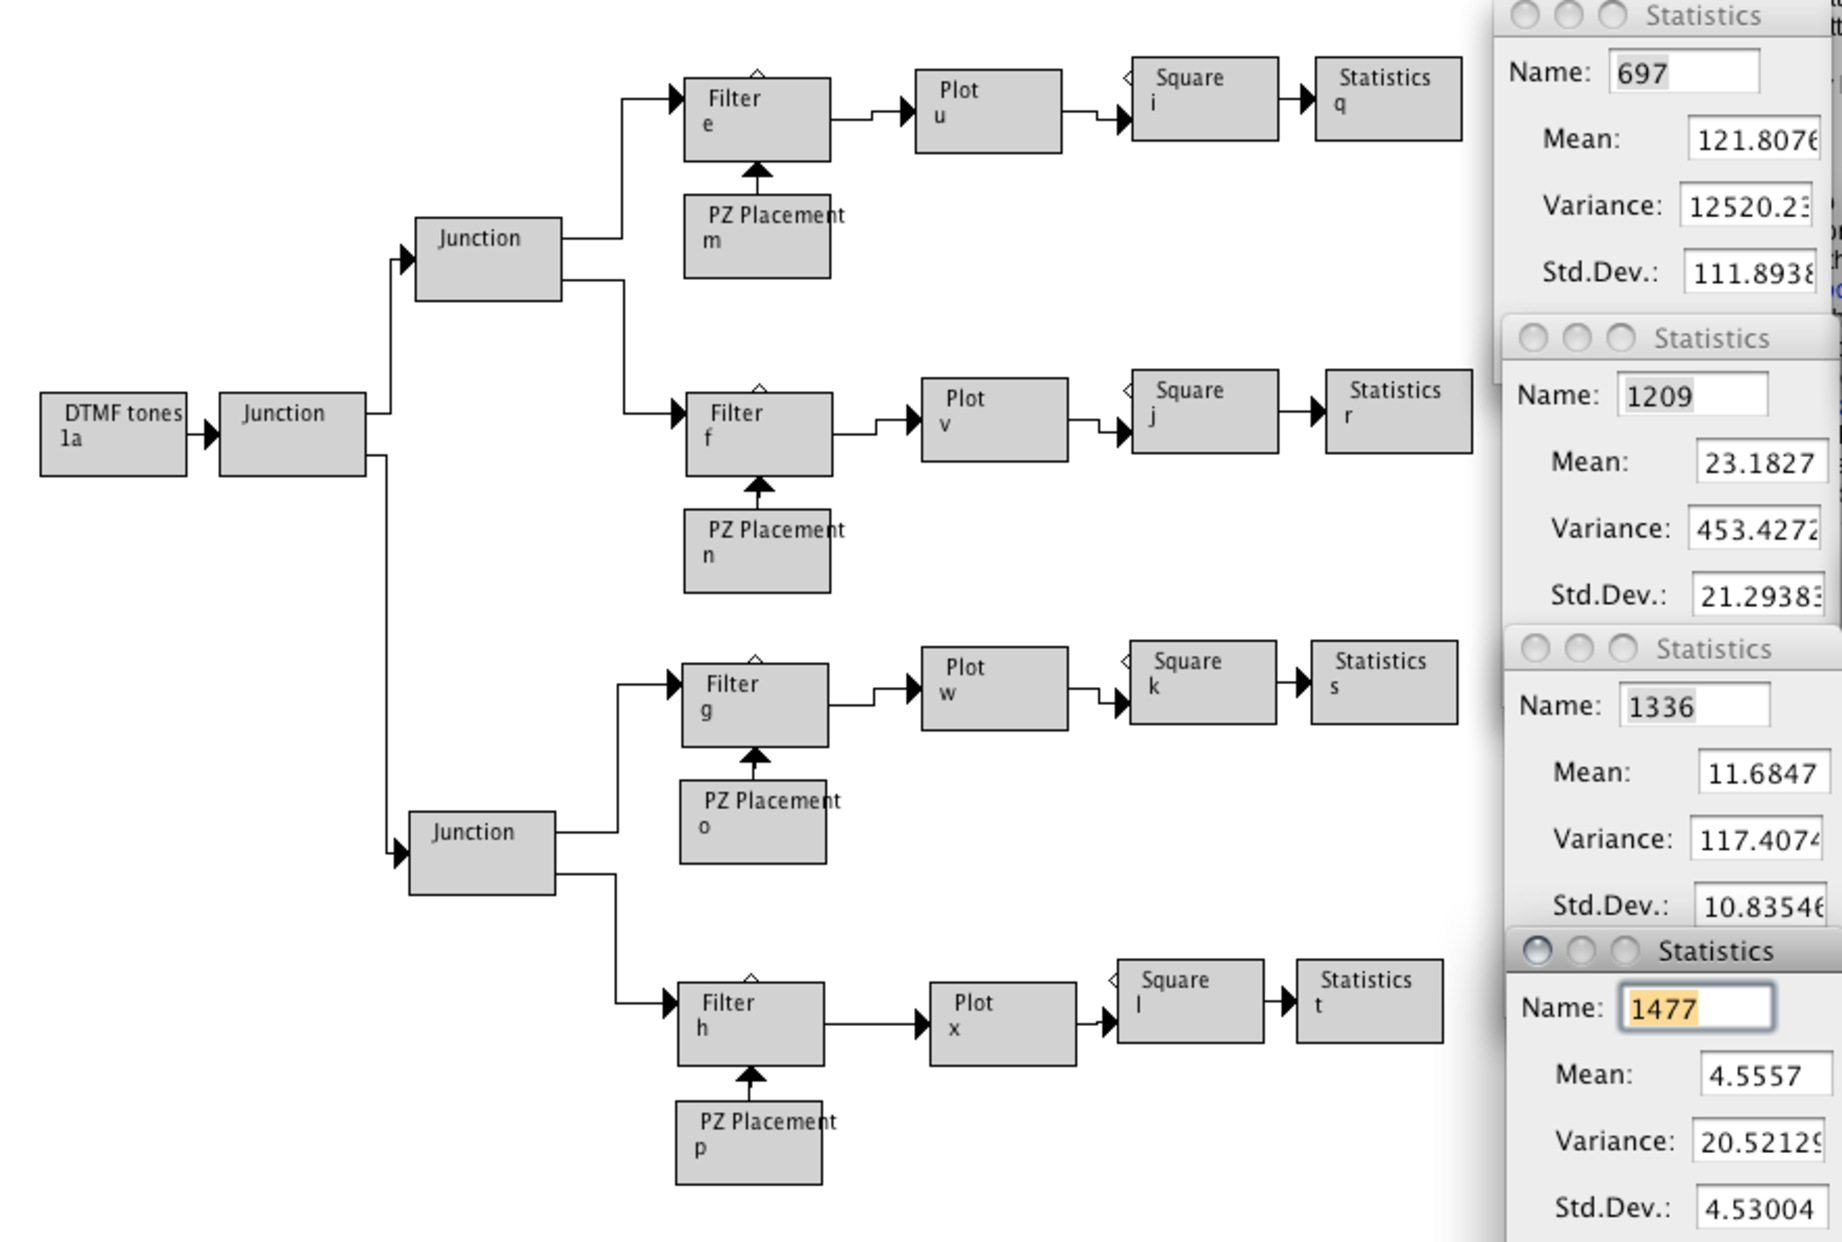
\includegraphics[width=6in]{lab7/screen}
  \end{center}
  \caption{Example filter bank layout.\label{fg:screen}}
\end{figure}

\paragraph{Step 2.4} Now we will assemble a filter bank. Your final layout 
should look something like Figure~\ref{fg:screen}. Pare down
your filter, etc. to the minimum set of blocks: \block{Filter},
\block{PZ Placement}, \block{Square}, and \block{Statistics}. Place four of these blocks down for
the four frequencies 697Hz, 1209Hz, 1336Hz, and 1477Hz; this will
allow us to recognize \button{1}, \button{2}, and \button{3}. Use
three \block{Junction}s to split the output of the \block{DTMF Tones}
block to send to four filters. Place the poles for each filter at the
same radius and the appropriate angles for each frequency (remember,
the \block{PZ Placement} block uses degrees for manual angle
entry). Name the \block{Statistics} blocks for the filters'
frequencies. Include a screen shot showing the output for
\block{DTMF Tones} button \button{2} in your report. What are the mean
squared values for each frequency for each of the \block{DTMF Tones}
buttons \button{1}, \button{2}, \button{3}, and \button{4}?  Would you
be able to use a simple pair of comparisons for each button to decode
which button was pressed? Why or why not?

% LocalWords:  WebQ MATLAB DSP
